Таким образом, постановка изучает оптимизацию как в локальном, так  глобальном поведением агента. Для вычисления исхода конкуренции используем подход, описанный в \cite{Bogdanov2023} для модели Бэрона-Фереджона. В этом случае определяющим свойством игрока является его очередь в формирование предложения. Введем обозначения $R$ для  выигрыша игрока, ходившего первым, и  $r$ - для второго.

Для определения оптимальный величины скидки первый игрок, рассчитает издержки неуспеха для  второго игрока состоящие из издержек в ожидание нового аукциона $P_\text{global}$ и еще один шаг торга $P_\text{local}= i \cdot \text{FC}$.

\begin{figure}[h]
    \centering
    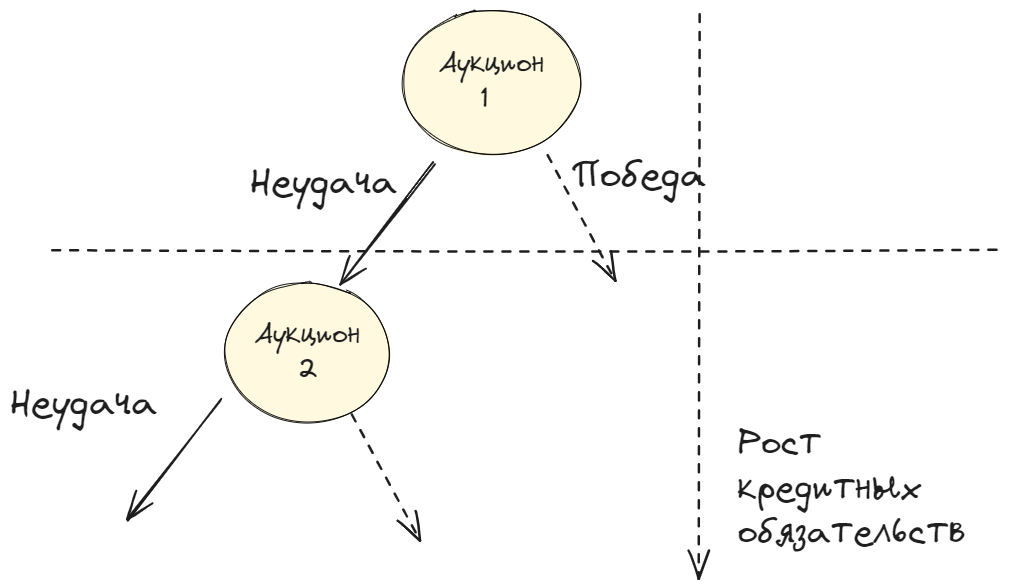
\includegraphics[width=0.5\textwidth]{assets/settings/dynamic.excalidraw.png}
    \caption{Агент при принятии решения учитывает возможность проигрыша в ряде раундов}
\end{figure}

Рис. 1. Соотношение между выигрышем сторон определяется через ликвидность продукта и ставку дисконтирования
Для определения Pglobal запишем матожидание по исходам в явной форме:
$$
    r  = - FC i   + 1/ 2 R  + 1/2  (- FC i   + 1/2  (R - FC i + 1/2 \dots)
$$
Телескопическая сумма может переписана как:
$$
    r = R (1/2 + 1/4 + \dots)  - FC i  (1 +1/2 +1/4 + \dots)
$$
Сокращая сумму в геометрическую прогрессию получим 
Pglobal=R-r = 2 * FC i  (2)
Тогда предложение первого поставщика будет определяться как минимум из максимальной скидки Mmax =K0-FC и суммы локальных и глобальных издержек:
M = min(Mmax,   Pglobal+Plocal) =min(K0 -FC,FCi(2+1)) (3),
Выводы 
ключевым для заключение сделки является право первого хода
кредитование пропорционально увеличивает стоимость поставки на величину ликвидности  и ставки рефинансирования i
